%\documentclass[slides]{beamer} %switch "slides" to "handout" for printing out
\documentclass[handout]{beamer}

%packages
%\usepackage{latexsym}
\usepackage{graphicx}
\usepackage{color}
\usepackage{amsmath}
\usepackage{dsfont}
\usepackage{placeins}
\usepackage{amssymb}
\usepackage{wasysym}
%\usepackage{abstract}
\usepackage{hyperref}
\usepackage{etoolbox}
\usepackage{datetime}
\usepackage{xcolor}
\usepackage{alphalph}
\usepackage[normalem]{ulem}
\settimeformat{ampmtime}

%\usepackage{pstricks,pst-node,pst-tree}

%\usepackage{algpseudocode}
%\usepackage{amsthm}
%\usepackage{hyperref}
%\usepackage{mathrsfs}
%\usepackage{amsfonts}
%\usepackage{bbding}
%\usepackage{listings}
%\usepackage{appendix}
%\usepackage[margin=1in]{geometry}
%\geometry{papersize={8.5in,11in},total={6.5in,9in}}
%\usepackage{cancel}
%\usepackage{algorithmic, algorithm}

\makeatletter
\def\maxwidth{ %
  \ifdim\Gin@nat@width>\linewidth
    \linewidth
  \else
    \Gin@nat@width
  \fi
}
\makeatother

\definecolor{fgcolor}{rgb}{0.345, 0.345, 0.345}
\newcommand{\hlnum}[1]{\textcolor[rgb]{0.686,0.059,0.569}{#1}}%
\newcommand{\hlstr}[1]{\textcolor[rgb]{0.192,0.494,0.8}{#1}}%
\newcommand{\hlcom}[1]{\textcolor[rgb]{0.678,0.584,0.686}{\textit{#1}}}%
\newcommand{\hlopt}[1]{\textcolor[rgb]{0,0,0}{#1}}%
\newcommand{\hlstd}[1]{\textcolor[rgb]{0.345,0.345,0.345}{#1}}%
\newcommand{\hlkwa}[1]{\textcolor[rgb]{0.161,0.373,0.58}{\textbf{#1}}}%
\newcommand{\hlkwb}[1]{\textcolor[rgb]{0.69,0.353,0.396}{#1}}%
\newcommand{\hlkwc}[1]{\textcolor[rgb]{0.333,0.667,0.333}{#1}}%
\newcommand{\hlkwd}[1]{\textcolor[rgb]{0.737,0.353,0.396}{\textbf{#1}}}%

\usepackage{framed}
\makeatletter
\newenvironment{kframe}{%
 \def\at@end@of@kframe{}%
 \ifinner\ifhmode%
  \def\at@end@of@kframe{\end{minipage}}%
  \begin{minipage}{\columnwidth}%
 \fi\fi%
 \def\FrameCommand##1{\hskip\@totalleftmargin \hskip-\fboxsep
 \colorbox{shadecolor}{##1}\hskip-\fboxsep
     % There is no \\@totalrightmargin, so:
     \hskip-\linewidth \hskip-\@totalleftmargin \hskip\columnwidth}%
 \MakeFramed {\advance\hsize-\width
   \@totalleftmargin\z@ \linewidth\hsize
   \@setminipage}}%
 {\par\unskip\endMakeFramed%
 \at@end@of@kframe}
\makeatother

\definecolor{shadecolor}{rgb}{.77, .77, .77}
\definecolor{messagecolor}{rgb}{0, 0, 0}
\definecolor{warningcolor}{rgb}{1, 0, 1}
\definecolor{errorcolor}{rgb}{1, 0, 0}
\newenvironment{knitrout}{}{} % an empty environment to be redefined in TeX

\usepackage{alltt}
\usepackage[T1]{fontenc}

\newcommand{\qu}[1]{``#1''}
\newcounter{probnum}
\setcounter{probnum}{1}

%create definition to allow local margin changes
\def\changemargin#1#2{\list{}{\rightmargin#2\leftmargin#1}\item[]}
\let\endchangemargin=\endlist 

%allow equations to span multiple pages
\allowdisplaybreaks

%define colors and color typesetting conveniences
\definecolor{gray}{rgb}{0.5,0.5,0.5}
\newcommand{\ingray}[1]{\color{gray}#1 \color{black}}
\newcommand{\ingrey}[1]{\ingray{#1}}
\definecolor{black}{rgb}{0,0,0}
\definecolor{white}{rgb}{1,1,1}
\definecolor{blue}{rgb}{0.5,0.5,1}
\newcommand{\inblue}[1]{\color{blue}#1 \color{black}}
\definecolor{green}{rgb}{0.133,0.545,0.133}
\newcommand{\ingreen}[1]{\color{green}#1 \color{black}}
\definecolor{yellow}{rgb}{1,1,0}
\newcommand{\inyellow}[1]{\color{yellow}#1 \color{black}}
\definecolor{orange}{rgb}{0.9,0.649,0}
\newcommand{\inorange}[1]{\color{orange}#1 \color{black}}
\definecolor{red}{rgb}{1,0.133,0.133}
\newcommand{\inred}[1]{\color{red}#1 \color{black}}
\definecolor{purple}{rgb}{0.58,0,0.827}
\newcommand{\inpurple}[1]{\color{purple}#1 \color{black}}
\definecolor{backgcode}{rgb}{0.97,0.97,0.8}
\definecolor{Brown}{cmyk}{0,0.81,1,0.60}
\definecolor{OliveGreen}{cmyk}{0.64,0,0.95,0.40}
\definecolor{CadetBlue}{cmyk}{0.62,0.57,0.23,0}

%define new math operators
\DeclareMathOperator*{\argmax}{arg\,max~}
\DeclareMathOperator*{\argmin}{arg\,min~}
\DeclareMathOperator*{\argsup}{arg\,sup~}
\DeclareMathOperator*{\arginf}{arg\,inf~}
\DeclareMathOperator*{\convolution}{\text{\Huge{$\ast$}}}
\newcommand{\infconv}[2]{\convolution^\infty_{#1 = 1} #2}
%true functions

%%%% GENERAL SHORTCUTS

%shortcuts for pure typesetting conveniences
\newcommand{\bv}[1]{\boldsymbol{#1}}

%shortcuts for compound constants
\newcommand{\BetaDistrConst}{\dfrac{\Gamma(\alpha + \beta)}{\Gamma(\alpha)\Gamma(\beta)}}
\newcommand{\NormDistrConst}{\dfrac{1}{\sqrt{2\pi\sigma^2}}}

%shortcuts for conventional symbols
\newcommand{\tsq}{\tau^2}
\newcommand{\tsqh}{\hat{\tau}^2}
\newcommand{\sigsq}{\sigma^2}
\newcommand{\sigsqsq}{\parens{\sigma^2}^2}
\newcommand{\sigsqovern}{\dfrac{\sigsq}{n}}
\newcommand{\tausq}{\tau^2}
\newcommand{\tausqalpha}{\tau^2_\alpha}
\newcommand{\tausqbeta}{\tau^2_\beta}
\newcommand{\tausqsigma}{\tau^2_\sigma}
\newcommand{\betasq}{\beta^2}
\newcommand{\sigsqvec}{\bv{\sigma}^2}
\newcommand{\sigsqhat}{\hat{\sigma}^2}
\newcommand{\sigsqhatmlebayes}{\sigsqhat_{\text{Bayes, MLE}}}
\newcommand{\sigsqhatmle}[1]{\sigsqhat_{#1, \text{MLE}}}
\newcommand{\bSigma}{\bv{\Sigma}}
\newcommand{\bSigmainv}{\bSigma^{-1}}
\newcommand{\thetavec}{\bv{\theta}}
\newcommand{\thetahat}{\hat{\theta}}
\newcommand{\thetahatmle}{\hat{\theta}_{\mathrm{MLE}}}
\newcommand{\thetavechatmle}{\hat{\thetavec}_{\mathrm{MLE}}}
\newcommand{\muhat}{\hat{\mu}}
\newcommand{\musq}{\mu^2}
\newcommand{\muvec}{\bv{\mu}}
\newcommand{\muhatmle}{\muhat_{\text{MLE}}}
\newcommand{\lambdahat}{\hat{\lambda}}
\newcommand{\lambdahatmle}{\lambdahat_{\text{MLE}}}
\newcommand{\etavec}{\bv{\eta}}
\newcommand{\alphavec}{\bv{\alpha}}
\newcommand{\minimaxdec}{\delta^*_{\mathrm{mm}}}
\newcommand{\ybar}{\bar{y}}
\newcommand{\xbar}{\bar{x}}
\newcommand{\Xbar}{\bar{X}}
\newcommand{\phat}{\hat{p}}
\newcommand{\Phat}{\hat{P}}
\newcommand{\Zbar}{\bar{Z}}
\newcommand{\iid}{~{\buildrel iid \over \sim}~}
\newcommand{\inddist}{~{\buildrel ind \over \sim}~}
\newcommand{\approxdist}{~{\buildrel approx \over \sim}~}
\newcommand{\equalsindist}{~{\buildrel d \over =}~}
\newcommand{\lik}[1]{\mathcal{L}\parens{#1}}
\newcommand{\loglik}[1]{\ell\parens{#1}}
\newcommand{\thetahatkminone}{\thetahat^{(k-1)}}
\newcommand{\thetahatkplusone}{\thetahat^{(k+1)}}
\newcommand{\thetahatk}{\thetahat^{(k)}}
\newcommand{\half}{\frac{1}{2}}
\newcommand{\third}{\frac{1}{3}}
\newcommand{\twothirds}{\frac{2}{3}}
\newcommand{\fourth}{\frac{1}{4}}
\newcommand{\fifth}{\frac{1}{5}}
\newcommand{\sixth}{\frac{1}{6}}

%shortcuts for vector and matrix notation
\newcommand{\A}{\bv{A}}
\newcommand{\At}{\A^T}
\newcommand{\Ainv}{\inverse{\A}}
\newcommand{\B}{\bv{B}}
\newcommand{\K}{\bv{K}}
\newcommand{\Kt}{\K^T}
\newcommand{\Kinv}{\inverse{K}}
\newcommand{\Kinvt}{(\Kinv)^T}
\newcommand{\M}{\bv{M}}
\newcommand{\Bt}{\B^T}
\newcommand{\Q}{\bv{Q}}
\newcommand{\Qt}{\Q^T}
\newcommand{\R}{\bv{R}}
\newcommand{\Rt}{\R^T}
\newcommand{\Z}{\bv{Z}}
\newcommand{\X}{\bv{X}}
\newcommand{\Xsub}{\X_{\text{(sub)}}}
\newcommand{\Xsubadj}{\X_{\text{(sub,adj)}}}
\newcommand{\I}{\bv{I}}
\newcommand{\Y}{\bv{Y}}
\newcommand{\sigsqI}{\sigsq\I}
\renewcommand{\P}{\bv{P}}
\newcommand{\Psub}{\P_{\text{(sub)}}}
\newcommand{\Pt}{\P^T}
\newcommand{\Pii}{P_{ii}}
\newcommand{\Pij}{P_{ij}}
\newcommand{\IminP}{(\I-\P)}
\newcommand{\Xt}{\bv{X}^T}
\newcommand{\XtX}{\Xt\X}
\newcommand{\XtXinv}{\parens{\Xt\X}^{-1}}
\newcommand{\XtXinvXt}{\XtXinv\Xt}
\newcommand{\XXtXinvXt}{\X\XtXinvXt}
\newcommand{\x}{\bv{x}}
\newcommand{\onevec}{\bv{1}}
\newcommand{\oneton}{1, \ldots, n}
\newcommand{\yoneton}{y_1, \ldots, y_n}
\newcommand{\yonetonorder}{y_{(1)}, \ldots, y_{(n)}}
\newcommand{\Yoneton}{Y_1, \ldots, Y_n}
\newcommand{\iinoneton}{i \in \braces{\oneton}}
\newcommand{\onetom}{1, \ldots, m}
\newcommand{\jinonetom}{j \in \braces{\onetom}}
\newcommand{\xoneton}{x_1, \ldots, x_n}
\newcommand{\Xoneton}{X_1, \ldots, X_n}
\newcommand{\xt}{\x^T}
\newcommand{\y}{\bv{y}}
\newcommand{\yt}{\y^T}
\renewcommand{\c}{\bv{c}}
\newcommand{\ct}{\c^T}
\newcommand{\tstar}{\bv{t}^*}
\renewcommand{\u}{\bv{u}}
\renewcommand{\v}{\bv{v}}
\renewcommand{\a}{\bv{a}}
\newcommand{\s}{\bv{s}}
\newcommand{\yadj}{\y_{\text{(adj)}}}
\newcommand{\xjadj}{\x_{j\text{(adj)}}}
\newcommand{\xjadjM}{\x_{j \perp M}}
\newcommand{\yhat}{\hat{y}}
\newcommand{\fhat}{\hat{f}}
\newcommand{\betahat}{\hat{\beta}}
\newcommand{\yhatsub}{\yhat_{\text{(sub)}}}
\newcommand{\yhatstar}{\yhat^*}
\newcommand{\yhatstarnew}{\yhatstar_{\text{new}}}
\newcommand{\z}{\bv{z}}
\newcommand{\zt}{\z^T}
\newcommand{\bb}{\bv{b}}
\newcommand{\bbt}{\bb^T}
\newcommand{\bbeta}{\bv{\beta}}
\newcommand{\beps}{\bv{\epsilon}}
\newcommand{\bepst}{\beps^T}
\newcommand{\e}{\bv{e}}
\newcommand{\Mofy}{\M(\y)}
\newcommand{\KofAlpha}{K(\alpha)}
\newcommand{\ellset}{\mathcal{L}}
\newcommand{\oneminalph}{1-\alpha}
\newcommand{\SSE}{\text{SSE}}
\newcommand{\SSEsub}{\text{SSE}_{\text{(sub)}}}
\newcommand{\MSE}{\text{MSE}}
\newcommand{\RMSE}{\text{RMSE}}
\newcommand{\SSR}{\text{SSR}}
\newcommand{\SST}{\text{SST}}
\newcommand{\JSest}{\delta_{\text{JS}}(\x)}
\newcommand{\Bayesest}{\delta_{\text{Bayes}}(\x)}
\newcommand{\EmpBayesest}{\delta_{\text{EmpBayes}}(\x)}
\newcommand{\BLUPest}{\delta_{\text{BLUP}}}
\newcommand{\MLEest}[1]{\hat{#1}_{\text{MLE}}}

%shortcuts for Linear Algebra stuff (i.e. vectors and matrices)
\newcommand{\twovec}[2]{\bracks{\begin{array}{c} #1 \\ #2 \end{array}}}
\newcommand{\threevec}[3]{\bracks{\begin{array}{c} #1 \\ #2 \\ #3 \end{array}}}
\newcommand{\fivevec}[5]{\bracks{\begin{array}{c} #1 \\ #2 \\ #3 \\ #4 \\ #5 \end{array}}}
\newcommand{\twobytwomat}[4]{\bracks{\begin{array}{cc} #1 & #2 \\ #3 & #4 \end{array}}}
\newcommand{\threebytwomat}[6]{\bracks{\begin{array}{cc} #1 & #2 \\ #3 & #4 \\ #5 & #6 \end{array}}}

%shortcuts for conventional compound symbols
\newcommand{\thetainthetas}{\theta \in \Theta}
\newcommand{\reals}{\mathbb{R}}
\newcommand{\complexes}{\mathbb{C}}
\newcommand{\rationals}{\mathbb{Q}}
\newcommand{\integers}{\mathbb{Z}}
\newcommand{\naturals}{\mathbb{N}}
\newcommand{\forallninN}{~~\forall n \in \naturals}
\newcommand{\forallxinN}[1]{~~\forall #1 \in \reals}
\newcommand{\matrixdims}[2]{\in \reals^{\,#1 \times #2}}
\newcommand{\inRn}[1]{\in \reals^{\,#1}}
\newcommand{\mathimplies}{\quad\Rightarrow\quad}
\newcommand{\mathlogicequiv}{\quad\Leftrightarrow\quad}
\newcommand{\eqncomment}[1]{\quad \text{(#1)}}
\newcommand{\limitn}{\lim_{n \rightarrow \infty}}
\newcommand{\limitN}{\lim_{N \rightarrow \infty}}
\newcommand{\limitd}{\lim_{d \rightarrow \infty}}
\newcommand{\limitt}{\lim_{t \rightarrow \infty}}
\newcommand{\limitsupn}{\limsup_{n \rightarrow \infty}~}
\newcommand{\limitinfn}{\liminf_{n \rightarrow \infty}~}
\newcommand{\limitk}{\lim_{k \rightarrow \infty}}
\newcommand{\limsupn}{\limsup_{n \rightarrow \infty}}
\newcommand{\limsupk}{\limsup_{k \rightarrow \infty}}
\newcommand{\floor}[1]{\left\lfloor #1 \right\rfloor}
\newcommand{\ceil}[1]{\left\lceil #1 \right\rceil}

%shortcuts for environments
\newcommand{\beqn}{\vspace{-0.25cm}\begin{eqnarray*}}
\newcommand{\eeqn}{\end{eqnarray*}}
\newcommand{\bneqn}{\vspace{-0.25cm}\begin{eqnarray}}
\newcommand{\eneqn}{\end{eqnarray}}

%shortcuts for mini environments
\newcommand{\parens}[1]{\left(#1\right)}
\newcommand{\squared}[1]{\parens{#1}^2}
\newcommand{\tothepow}[2]{\parens{#1}^{#2}}
\newcommand{\prob}[1]{\mathbb{P}\parens{#1}}
\newcommand{\cprob}[2]{\prob{#1~|~#2}}
\newcommand{\littleo}[1]{o\parens{#1}}
\newcommand{\bigo}[1]{O\parens{#1}}
\newcommand{\Lp}[1]{\mathbb{L}^{#1}}
\renewcommand{\arcsin}[1]{\text{arcsin}\parens{#1}}
\newcommand{\prodonen}[2]{\bracks{\prod_{#1=1}^n #2}}
\newcommand{\mysum}[4]{\sum_{#1=#2}^{#3} #4}
\newcommand{\sumonen}[2]{\sum_{#1=1}^n #2}
\newcommand{\sumionen}[1]{\sumonen{i}{#1}}
\newcommand{\infsum}[2]{\sum_{#1=1}^\infty #2}
\newcommand{\infprod}[2]{\prod_{#1=1}^\infty #2}
\newcommand{\infunion}[2]{\bigcup_{#1=1}^\infty #2}
\newcommand{\infinter}[2]{\bigcap_{#1=1}^\infty #2}
\newcommand{\infintegral}[2]{\int^\infty_{-\infty} #2 ~\text{d}#1}
\newcommand{\supthetas}[1]{\sup_{\thetainthetas}\braces{#1}}
\newcommand{\bracks}[1]{\left[#1\right]}
\newcommand{\braces}[1]{\left\{#1\right\}}
\newcommand{\angbraces}[1]{\left<#1\right>}
\newcommand{\set}[1]{\left\{#1\right\}}
\newcommand{\abss}[1]{\left|#1\right|}
\newcommand{\norm}[1]{\left|\left|#1\right|\right|}
\newcommand{\normsq}[1]{\norm{#1}^2}
\newcommand{\inverse}[1]{\parens{#1}^{-1}}
\newcommand{\rowof}[2]{\parens{#1}_{#2\cdot}}

%shortcuts for functionals
\newcommand{\realcomp}[1]{\text{Re}\bracks{#1}}
\newcommand{\imagcomp}[1]{\text{Im}\bracks{#1}}
\newcommand{\range}[1]{\text{range}\bracks{#1}}
\newcommand{\colsp}[1]{\text{colsp}\bracks{#1}}
\newcommand{\rowsp}[1]{\text{rowsp}\bracks{#1}}
\newcommand{\tr}[1]{\text{tr}\bracks{#1}}
\newcommand{\rank}[1]{\text{rank}\bracks{#1}}
\newcommand{\proj}[2]{\text{Proj}_{#1}\bracks{#2}}
\newcommand{\projcolspX}[1]{\text{Proj}_{\colsp{\X}}\bracks{#1}}
\newcommand{\median}[1]{\text{median}\bracks{#1}}
\newcommand{\mean}[1]{\text{mean}\bracks{#1}}
\newcommand{\dime}[1]{\text{dim}\bracks{#1}}
\renewcommand{\det}[1]{\text{det}\bracks{#1}}
\newcommand{\expe}[1]{\mathbb{E}\bracks{#1}}
\newcommand{\cexpe}[2]{\expe{#1~|~#2}}
\newcommand{\expeabs}[1]{\expe{\abss{#1}}}
\newcommand{\expesub}[2]{\mathbb{E}_{#1}\bracks{#2}}
\newcommand{\indic}[1]{\mathds{1}_{#1}}
\newcommand{\var}[1]{\mathbb{V}\text{ar}\bracks{#1}}
\newcommand{\cov}[2]{\mathbb{C}\text{ov}\bracks{#1, #2}}
\newcommand{\corr}[2]{\text{Corr}\bracks{#1, #2}}
\newcommand{\se}[1]{\mathbb{S}\text{E}\bracks{#1}}
\newcommand{\seest}[1]{\hat{\text{SE}}\bracks{#1}}
\newcommand{\bias}[1]{\text{Bias}\bracks{#1}}
\newcommand{\derivop}[2]{\dfrac{\text{d}}{\text{d} #1}\bracks{#2}}
\newcommand{\partialop}[2]{\dfrac{\partial}{\partial #1}\bracks{#2}}
\newcommand{\secpartialop}[2]{\dfrac{\partial^2}{\partial #1^2}\bracks{#2}}
\newcommand{\mixpartialop}[3]{\dfrac{\partial^2}{\partial #1 \partial #2}\bracks{#3}}

%shortcuts for functions
\renewcommand{\exp}[1]{\mathrm{exp}\parens{#1}}
\renewcommand{\cos}[1]{\text{cos}\parens{#1}}
\renewcommand{\sin}[1]{\text{sin}\parens{#1}}
\newcommand{\sign}[1]{\text{sign}\parens{#1}}
\newcommand{\are}[1]{\mathrm{ARE}\parens{#1}}
\newcommand{\natlog}[1]{\ln\parens{#1}}
\newcommand{\oneover}[1]{\frac{1}{#1}}
\newcommand{\overtwo}[1]{\frac{#1}{2}}
\newcommand{\overn}[1]{\frac{#1}{n}}
\newcommand{\oneoversqrt}[1]{\oneover{\sqrt{#1}}}
\newcommand{\sqd}[1]{\parens{#1}^2}
\newcommand{\loss}[1]{\ell\parens{\theta, #1}}
\newcommand{\losstwo}[2]{\ell\parens{#1, #2}}
\newcommand{\cf}{\phi(t)}

%English language specific shortcuts
\newcommand{\ie}{\textit{i.e.} }
\newcommand{\AKA}{\textit{AKA} }
\renewcommand{\iff}{\textit{iff}}
\newcommand{\eg}{\textit{e.g.} }
\newcommand{\st}{\textit{s.t.} }
\newcommand{\wrt}{\textit{w.r.t.} }
\newcommand{\mathst}{~~\text{\st}~~}
\newcommand{\mathand}{~~\text{and}~~}
\newcommand{\ala}{\textit{a la} }
\newcommand{\ppp}{posterior predictive p-value}
\newcommand{\dd}{dataset-to-dataset}

%shortcuts for distribution titles
\newcommand{\logistic}[2]{\mathrm{Logistic}\parens{#1,\,#2}}
\newcommand{\bernoulli}[1]{\mathrm{Bernoulli}\parens{#1}}
\newcommand{\betanot}[2]{\mathrm{Beta}\parens{#1,\,#2}}
\newcommand{\stdbetanot}{\betanot{\alpha}{\beta}}
\newcommand{\multnormnot}[3]{\mathcal{N}_{#1}\parens{#2,\,#3}}
\newcommand{\normnot}[2]{\mathcal{N}\parens{#1,\,#2}}
\newcommand{\classicnormnot}{\normnot{\mu}{\sigsq}}
\newcommand{\stdnormnot}{\normnot{0}{1}}
\newcommand{\uniformdiscrete}[1]{\mathrm{Uniform}\parens{\braces{#1}}}
\newcommand{\uniform}[2]{\mathrm{U}\parens{#1,\,#2}}
\newcommand{\stduniform}{\uniform{0}{1}}
\newcommand{\geometric}[1]{\mathrm{Geometric}\parens{#1}}
\newcommand{\hypergeometric}[3]{\mathrm{Hypergeometric}\parens{#1,\,#2,\,#3}}
\newcommand{\exponential}[1]{\mathrm{Exp}\parens{#1}}
\newcommand{\gammadist}[2]{\mathrm{Gamma}\parens{#1, #2}}
\newcommand{\poisson}[1]{\mathrm{Poisson}\parens{#1}}
\newcommand{\binomial}[2]{\mathrm{Binomial}\parens{#1,\,#2}}
\newcommand{\negbin}[2]{\mathrm{NegBin}\parens{#1,\,#2}}
\newcommand{\rayleigh}[1]{\mathrm{Rayleigh}\parens{#1}}
\newcommand{\multinomial}[2]{\mathrm{Multinomial}\parens{#1,\,#2}}
\newcommand{\gammanot}[2]{\mathrm{Gamma}\parens{#1,\,#2}}
\newcommand{\cauchynot}[2]{\text{Cauchy}\parens{#1,\,#2}}
\newcommand{\invchisqnot}[1]{\text{Inv}\chisq{#1}}
\newcommand{\invscaledchisqnot}[2]{\text{ScaledInv}\ncchisq{#1}{#2}}
\newcommand{\invgammanot}[2]{\text{InvGamma}\parens{#1,\,#2}}
\newcommand{\chisq}[1]{\chi^2_{#1}}
\newcommand{\ncchisq}[2]{\chi^2_{#1}\parens{#2}}
\newcommand{\ncF}[3]{F_{#1,#2}\parens{#3}}

%shortcuts for PDF's of common distributions
\newcommand{\logisticpdf}[3]{\oneover{#3}\dfrac{\exp{-\dfrac{#1 - #2}{#3}}}{\parens{1+\exp{-\dfrac{#1 - #2}{#3}}}^2}}
\newcommand{\betapdf}[3]{\dfrac{\Gamma(#2 + #3)}{\Gamma(#2)\Gamma(#3)}#1^{#2-1} (1-#1)^{#3-1}}
\newcommand{\normpdf}[3]{\frac{1}{\sqrt{2\pi#3}}\exp{-\frac{1}{2#3}(#1 - #2)^2}}
\newcommand{\normpdfvarone}[2]{\dfrac{1}{\sqrt{2\pi}}e^{-\half(#1 - #2)^2}}
\newcommand{\chisqpdf}[2]{\dfrac{1}{2^{#2/2}\Gamma(#2/2)}\; {#1}^{#2/2-1} e^{-#1/2}}
\newcommand{\invchisqpdf}[2]{\dfrac{2^{-\overtwo{#1}}}{\Gamma(#2/2)}\,{#1}^{-\overtwo{#2}-1}  e^{-\oneover{2 #1}}}
\newcommand{\exponentialpdf}[2]{#2\exp{-#2#1}}
\newcommand{\poissonpdf}[2]{\dfrac{e^{-#1} #1^{#2}}{#2!}}
\newcommand{\binomialpdf}[3]{\binom{#2}{#1}#3^{#1}(1-#3)^{#2-#1}}
\newcommand{\rayleighpdf}[2]{\dfrac{#1}{#2^2}\exp{-\dfrac{#1^2}{2 #2^2}}}
\newcommand{\gammapdf}[3]{\dfrac{#3^#2}{\Gamma\parens{#2}}#1^{#2-1}\exp{-#3 #1}}
\newcommand{\cauchypdf}[3]{\oneover{\pi} \dfrac{#3}{\parens{#1-#2}^2 + #3^2}}
\newcommand{\Gammaf}[1]{\Gamma\parens{#1}}

%shortcuts for miscellaneous typesetting conveniences
\newcommand{\notesref}[1]{\marginpar{\color{gray}\tt #1\color{black}}}

%%%% DOMAIN-SPECIFIC SHORTCUTS

%Real analysis related shortcuts
\newcommand{\zeroonecl}{\bracks{0,1}}
\newcommand{\forallepsgrzero}{\forall \epsilon > 0~~}
\newcommand{\lessthaneps}{< \epsilon}
\newcommand{\fraccomp}[1]{\text{frac}\bracks{#1}}

%Bayesian related shortcuts
\newcommand{\yrep}{y^{\text{rep}}}
\newcommand{\yrepisq}{(\yrep_i)^2}
\newcommand{\yrepvec}{\bv{y}^{\text{rep}}}


%Probability shortcuts
\newcommand{\SigField}{\mathcal{F}}
\newcommand{\ProbMap}{\mathcal{P}}
\newcommand{\probtrinity}{\parens{\Omega, \SigField, \ProbMap}}
\newcommand{\convp}{~{\buildrel p \over \rightarrow}~}
\newcommand{\convLp}[1]{~{\buildrel \Lp{#1} \over \rightarrow}~}
\newcommand{\nconvp}{~{\buildrel p \over \nrightarrow}~}
\newcommand{\convae}{~{\buildrel a.e. \over \longrightarrow}~}
\newcommand{\convau}{~{\buildrel a.u. \over \longrightarrow}~}
\newcommand{\nconvau}{~{\buildrel a.u. \over \nrightarrow}~}
\newcommand{\nconvae}{~{\buildrel a.e. \over \nrightarrow}~}
\newcommand{\convd}{~{\buildrel \mathcal{D} \over \rightarrow}~}
\newcommand{\nconvd}{~{\buildrel \mathcal{D} \over \nrightarrow}~}
\newcommand{\withprob}{~~\text{w.p.}~~}
\newcommand{\io}{~~\text{i.o.}}

\newcommand{\Acl}{\bar{A}}
\newcommand{\ENcl}{\bar{E}_N}
\newcommand{\diam}[1]{\text{diam}\parens{#1}}

\newcommand{\taua}{\tau_a}

\newcommand{\myint}[4]{\int_{#2}^{#3} #4 \,\text{d}#1}
\newcommand{\laplacet}[1]{\mathscr{L}\bracks{#1}}
\newcommand{\laplaceinvt}[1]{\mathscr{L}^{-1}\bracks{#1}}
%\renewcommand{\min}[1]{\text{min}\braces{#1}}
%\renewcommand{\max}[1]{\text{max}\braces{#1}}

\newcommand{\Vbar}[1]{\bar{V}\parens{#1}}
\newcommand{\expnegrtau}{\exp{-r\tau}}
\newcommand{\errorrv}{\mathcal{E}}

%%% problem typesetting

%%% problem typesetting
\definecolor{darkgrey}{rgb}{0.10,0.10,0.9}
%
%\newcommand{\problem}[1]{\noindent \colorbox{black}{{\color{yellow} \large{\textsf{\textbf{Problem \arabic{probnum}}}}~}} \addtocounter{probnum}{1} \vspace{0.2cm} \\ \iftoggle{professormode}{}{\color{darkgrey}} #1}
%
%\newcommand{\easysubproblem}[1]{\ingreen{\item} \iftoggle{professormode}{}{\color{darkgrey}} [easy] #1 \color{black} }
%\newcommand{\intermediatesubproblem}[1]{\inorange{\item} \iftoggle{professormode}{}{\color{darkgrey}} [harder] #1 \color{black} }
%\newcommand{\hardsubproblem}[1]{\inred{\item} \iftoggle{professormode}{}{\color{darkgrey}} [difficult] #1 \color{black} }
%\newcommand{\extracreditsubproblem}[1]{\inpurple{\item} \iftoggle{professormode}{}{\color{darkgrey}} [E.C.] #1 \color{black} }


%\newcommand{\spc}[1]{\iftoggle{professormode}{\\ \vspace{#1cm}}{\\ \vspace{-0.3cm}}}

%\makeatletter
%\newalphalph{\alphmult}[mult]{\@alph}{26}
%\renewcommand{\labelenumi}{(\alphmult{\value{enumi}})}

\newcommand{\support}[1]{\text{Supp}\bracks{#1}}
%\newcommand{\mode}[1]{\text{Mode}\bracks{#1}}
\newcommand{\IQR}[1]{\text{IQR}\bracks{#1}}
\newcommand{\quantile}[2]{\text{Quantile}\bracks{#1,\,#2}}


%presentation preamble
\usetheme{progressbar}
\usecolortheme{progressbar} 
\usefonttheme{progressbar} 
\useoutertheme{progressbar}
\useinnertheme{progressbar}

\title[Lec 1]{Predictive Analytics Lecture 2}
\institute[Wharton, Statistics]{Stat 422/722\\ at The Wharton School of the University of Pennsylvania}
\date{January 17 \& 18, 2017}

\author{Adam Kapelner}


\begin{document}

%immediately create a title page
\frame{\titlepage}

\section{LM Inference via MLE and Correlation $\not \Rightarrow$ Causation}




\begin{frame}\frametitle{No Inference Possible as of Now}

We haven't spoken about $t$ or $F$ tests. Why is that? \\~\\ \pause 

In order to have inference, we need to make explicit random variable model assumptions

\beqn
Y \sim g( \beta_0 + \beta_1 x_1 + \ldots + \beta_p x_p, \sigsq, \ldots)
\eeqn

must be assumed to be something like

\beqn
Y \sim \normnot{\beta_0 + \beta_1 x_1 + \ldots + \beta_p x_p}{\sigsq}
\eeqn

Is this a reasonable thing to do?
	
\end{frame}

\begin{frame}\frametitle{Back to Modeling}

We said before that our model for $Y$ was

\beqn
Y = f(x_1, \ldots, x_p) + \errorrv
\eeqn

assuming we can know the model, there still is $\errorrv$. Where does it come from? According to determinism a la Laplace, if one knew all the causal information, there would be no error

\beqn
y = t(z_1, z_2, \ldots)
\eeqn

i.e $t$ is the deterministic true mathematical model. %Consider the cigarette example .%where the response is completely explained by the \emph{causal} variables $c_1, c_2, \ldots$. Causal is usually defined as a variable that affects the response variable that one can \qu{manipulate}. 

	
\end{frame}

\begin{frame}\frametitle{}

\begin{figure}
\centering
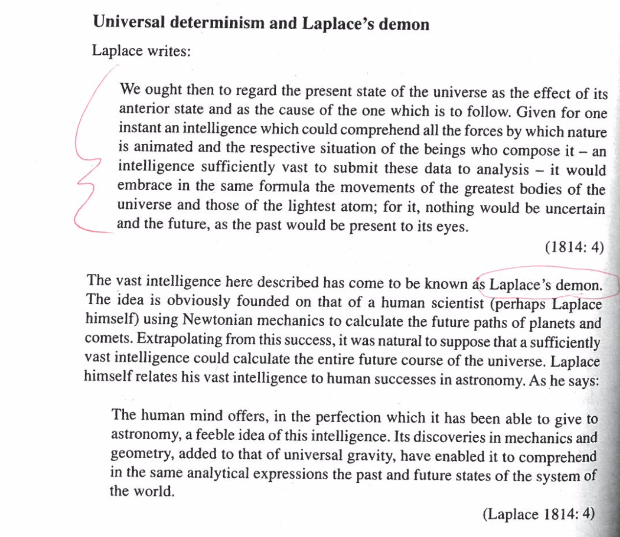
\includegraphics[width=3.5in]{laplace.png}
\end{figure}

\end{frame}

\begin{frame}\frametitle{Example Lung Cancer Causal Model}

\begin{figure}
\centering
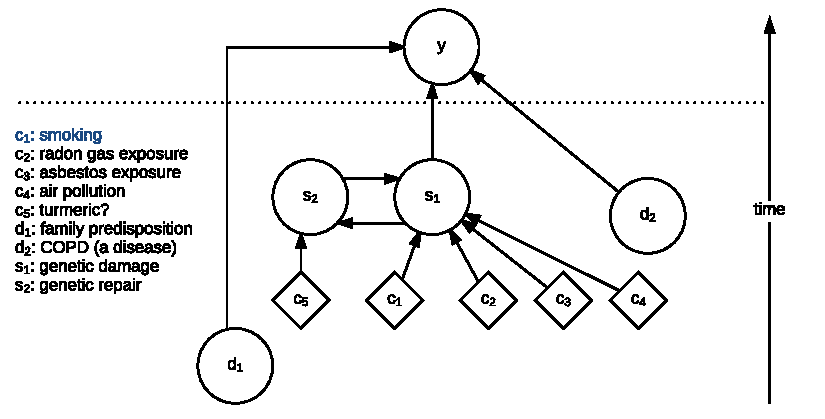
\includegraphics[width=3.8in]{cigarettes}
\end{figure}

\small
Arrows represent causal directions and diamond boxes represent \qu{manipulable} variables (more on this soon). \pause  What functions for the response would be deterministic?

\beqn
y = t(\pause d_1, d_2, s_1), y = t(d_1, d_2, s_2, \pause c_1, c_2, c_3, c_4), y = t(d_1, d_2, c_1, c_2, c_3, c_4, \pause c_5) \\
\eeqn
%%http://www.webmd.com/lung-cancer/guide/lung-cancer-causes#3
\end{frame}

\begin{frame}\frametitle{The Root Cause of Randomness}

\small
But let's say we only have information about $c_1$ (a contributory cause, one among many co-occurrent causes). Since we don't have all the inputs (nor the information of the states of the co-occurent causes), we cannot be sure of $y$. Hence we'll employ a statistical model,

\beqn
Y \sim \pause \bernoulli{f(c_1)}
\eeqn

where we saw before that $f(c_1 = 1) = 16\%$ and $f(c_1 = 0) = 0.4\%$ (probabilistic causation). Thus, the response is stochastic only because we lack information. For regression,\\~\\

\beqn
Y = f(x_1, \ldots, x_p) + \underbrace{t(z_1, z_2, \ldots) - f(x_1, \ldots, x_p)}_{\substack{\pause \errorrv \\ \pause \text{(i.e. the \qu{noise} is due to ignorance)}}}
\eeqn

\footnotesize
Note... some believe that there is still intrinsic randomness in the universe even with all relevant information known. But we are punting on the actual philosophy...
	
\end{frame}


\begin{frame}\frametitle{$t$ is Difficult to Model}

In order to get $t$, you'll need to know all these functions explicitly:

\beqn
y &=& t_y(\pause d_1, d_2, s_1) \\
s_1 &=& t_{s_1}(c_1, c_2, c_3,c_4,s_2) \\
s_2 &=& f_{s_2}(c_5, s_1)
\eeqn

which means that even if you know all the values of variables, you may not be able to properly model the response since you do not know the functional forms $t_y$, $t_{s_1}$ and $t_{s_2}$.

\end{frame}


\begin{frame}\frametitle{A \qu{Nice} Type of Ignorance}

\begin{figure}
\centering
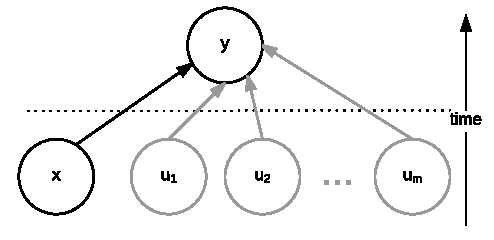
\includegraphics[width=2.5in]{nice_ignorance}
\end{figure}

\small
In the situation where the true model is 

\beqn
y = g(x) + h_1(u_1) + h_2(u_2) + \ldots + h_m(u_m)
\eeqn

and $x$ is observed but $u_1, \ldots, u_m$ are unseen.

\beqn
h_1(u_1) + h_2(u_2) + \ldots + h_m(u_m) \convd \normnot{\sum_{k=1}^m \mu_k}{\sum_{k=1}^m \sigsq_k}
\eeqn

as the number of unseen variables increase (central limit theorem).

\end{frame}

\begin{frame}\frametitle{The Normal Homoskedastic Error Model}

Let $c = \sum_{k=1}^m \mu_k$ and $\sigsq = \sum_{k=1}^m \sigsq_k$, then

\beqn
y = \underbrace{g(x) + c}_{f(x)} + \errorrv, \quad \text{s.t.} \quad \errorrv =  \sum_{k=1}^m h_k(u_k) - c \sim \normnot{0}{\sigsq}
\eeqn

\begin{figure}
\centering
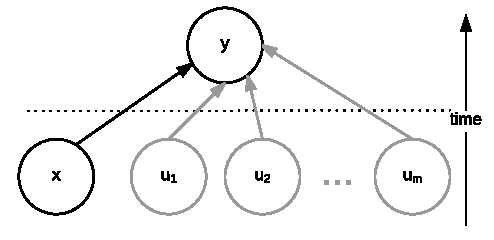
\includegraphics[width=1.5in]{nice_ignorance}
\end{figure}

Also, since $x$ does not affect the other variables in any way, it cannot have an influence on their spread, hence $\sigsq$ is not a function of $x$. Thus the error spread is the same everywhere across the range of $x$ (homoskedasticity).

\end{frame}

\begin{frame}\frametitle{Parametric Worldview}

We are back to the fundamental statistical problem, $Y = f(x) + \errorrv$ where now we are more \qu{okay} with the noise being normal and homoskedastic for all $x$.\\~\\

We now invoke the parametric worldview. Within that parametric worldview, we will buy into the linear model. Thus,

\beqn
Y \sim \normnot{\beta_0 + \beta_1 x_1 + \ldots + \beta_p x_p}{\sigsq}
\eeqn

But there is one more assumption...
	
\end{frame}

\begin{frame}\frametitle{Independence}

We now assume that each response is independent of every other response. \footnotesize Second person:

\begin{minipage}{0.55\textwidth}

\begin{figure}
\centering
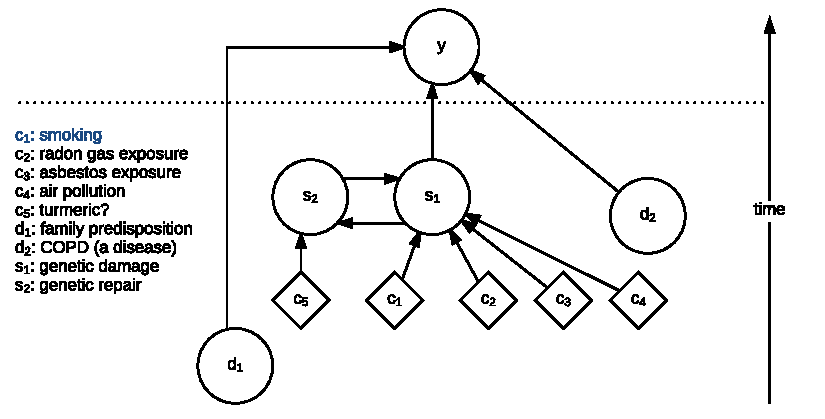
\includegraphics[width=2.1in]{cigarettes}
\end{figure}
First person:
\begin{figure}
\centering
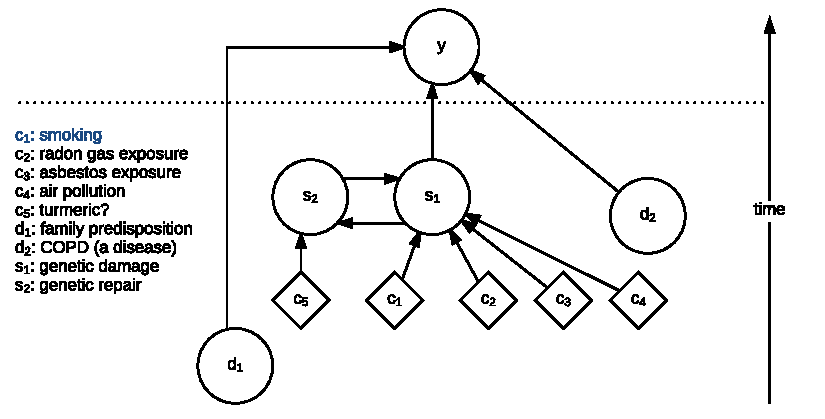
\includegraphics[width=2.1in]{cigarettes}
\end{figure}
\end{minipage}
\begin{minipage}{0.35\textwidth}
\normalsize
No effect of first person's $y_1$ (nor any of the unobserved variables which generate the $\errorrv_1$) on the second person's $y$ (or $\errorrv_2$). \\~\\ \pause

If there are, we need to observe them and rotate them into our estimate of $f(x)$. Examples for this cigarette case?
\end{minipage}

\end{frame}


\begin{frame}\frametitle{The Classic OLS Assumptions}

Preassuming

\begin{itemize}
\item linearity (the parametric assumption)
\end{itemize}

we then	further assume

\begin{itemize}
\item independence (most important)
\item homoskedasticity (less important)
\item normality of $\errorrv$ (least important if $n$ is large)
\end{itemize}

in order to get inference.

\end{frame}

\begin{frame}\frametitle{A Different Means of Estimation}

\small
Last time, we were working on creating a fit $\fhat$ that means we need estimates of all the parameters:

\beqn
\fhat(x_1, x_2, \ldots, x_p) = \betahat_0 + \betahat_1 x_1 + \ldots + \betahat_p x_p
\eeqn

where the unknown parameters were $\beta_0, \beta_1, \ldots, \beta_p$. Our strategy last time was to minimize SSE via a calculus to obtain $\braces{\betahat_0, \betahat_1,  \ldots, \betahat_p}$. \pause Why was this arbitrary? \\~\\

Given the three new assumptions (that it's not too much of a stretch to buy into usually), we now have a completely specified joint probability distribution for our observed data,

\beqn
\cprob{Y_1 = y_1, Y_2 = y_2, \ldots, Y_n = y_n}{\X_1 = \x_1, \X_2 = \x_2, \ldots, \X_n = \x_n}
\eeqn
	
where $\x_i := \bracks{x_{i1}, x_{i2}, \ldots, x_{ip}}$ i.e. the vector of all known measurements / covariates.

\end{frame}


\begin{frame}\frametitle{What's a probability? What's a likelihood? }

\small
In general, a parametric density function / mass function of a r.v. looks like the following:

\beqn
\prob{x; \theta} = \ldots
\eeqn

where $\theta$ are the tuning knobs on the model. We ask the question \qu{what's the probability of this realization $x$ (the data) assuming the density was parameterized at $\theta$}? Now we ask the inverse question:

\beqn
\lik{\theta; x}= \ldots
\eeqn

that is \qu{what's the likelihood of these parameters assuming we saw $x$ (the data) come out the way it did}? The $\lik{}$ denotes the \emph{likelihood function}. Of course, probability and likelihood are exactly the same numerically, 

\beqn
\prob{x; \theta} = \lik{\theta; x}= \ldots
\eeqn

but conceptually they couldn't be further apart!
	
\end{frame}

\begin{frame}\frametitle{Maximum Likelihood Estimation (MLE)}

\small
Why not just ask the very common-sense question, what $\theta$ maximizes the probability of seeing what we observe? That would be a good guess as to what $\theta$ is.\pause 

\beqn
\thetahat := \argmax_{\theta \in \Theta} \braces{\lik{\theta; x}}
\eeqn

where $\Theta$ represents the space the parameter lives in. In our situation, $\Theta$ represents \pause all real numbers in $p$ dimensions. Let's do this in our example. The first step:


\beqn
&&\cprob{Y_1 = y_1, Y_2 = y_2, \ldots, Y_n = y_n}{\X_1 = \x_1, \X_2 = \x_2, \ldots, \X_n = \x_n} \\
&=& \prod_{i=1}^n \cprob{Y_i = y_i}{\X_1 = \x_i}
\eeqn

How so? \pause Each observation is independent of every other. Recall $\prob{ABC} = \prob{A}\prob{B}\prob{C}$ if $A$, $B$ and $C$ are independent.
	
\end{frame}


\begin{frame}\frametitle{MLE of the Linear Model Parameters}

\small
We can continue,

\beqn
&=& \prod_{i=1}^n \cprob{Y_i = y_i}{\X_1 = \x_i} \\ 
&=& \prod_{i=1}^n \oneoversqrt{2\pi \sigsq} \exp{-\oneover{2\sigsq} \squared{y - \cexpe{Y_i}{\X_i}}}
\eeqn

How? \pause Normality and homoskedasticity of $\errorrv$.

\beqn
&=& \prod_{i=1}^n \oneoversqrt{2\pi \sigsq} \exp{-\oneover{2\sigsq} \squared{y - (\beta_0 + \beta_1 x_{i1}+ \ldots + \beta_p x_{ip})}} \\ \pause
\eeqn

How? \pause Linearity of $\cexpe{Y_i}{\X_i}$. Now we wish to maximize the above over all possible $\beta_0, \beta_1, \ldots, \beta_p$.


	
\end{frame}

\begin{frame}\frametitle{MLE of the Linear Model Parameters}

\small
Then, by some precalc tricks,

\beqn
&=& \prod_{i=1}^n \oneoversqrt{2\pi \sigsq} \exp{-\oneover{2\sigsq} \errorrv_i^2} \\ \pause
&=& \tothepow{\oneoversqrt{2\pi \sigsq}}{n} \exp{\sum_{i=1}^n -\oneover{2\sigsq} \errorrv_i^2} \\ \pause
&=& \tothepow{\oneoversqrt{2\pi \sigsq}}{n} \exp{-\oneover{2\sigsq} \sum_{i=1}^n \errorrv_i^2} 
\eeqn

Pick $\braces{\betahat_0, \betahat_1,  \ldots, \betahat_p, \sigsqhat}$ such that the above is minimized. The solutions are called the \qu{maximum likelihood estimates (MLE's)}.
	
\end{frame}

\begin{frame}\frametitle{Amazing coincidence}

Using calculus, the solution to $\braces{\betahat_0, \betahat_1,  \ldots, \betahat_p}$ is equivalent to minimizing SSE... What a coincidence!! \\~\\

\small
Note: $\sigsqhat = \oneover{n} SSE$

\end{frame}


\begin{frame}\frametitle{The Likelihood Ratio (LR)}

%\small
Imagine two models: (a) the \qu{full} model where $\theta \in \Theta$ and (b) a reduced model where $\theta \in \Theta_R \subset \Theta$. The reduced space has $q$ less degrees of freedom for $\theta$ to operate. Consider the ratio of the likelihoods

\beqn
LR :=
%
\displaystyle \max_{\theta \in \Theta} \lik{\theta; x}
%
/
%
\displaystyle \max_{\theta \in \Theta_R}  \lik{\theta; x}
%
\eeqn

representing how much more probable the full model is over the restricted model. But is this is this increase in probability \emph{statistically significant}? It turns out as $n$ gets large and under pretty forgiving conditions,

\beqn
Q := 2 \natlog{LR} \convd \chisq{q}
\eeqn


\end{frame}

\begin{frame}\frametitle{Testing the Simple Reduced Model}

Let's test our \qu{naive model} from Lecture 1 (always predicting $\yhat = \ybar$) versus having a model having many predictors in a linear model.

\beqn
LR &=& \frac{
\displaystyle \max_{\beta_0, \beta_1, \ldots, \beta_p, \sigsq} 
\lik{\beta_0, \beta_1, \ldots, \beta_p; y_1, \ldots, y_n, \x_1, \ldots, \x_n}
}{
\displaystyle \max_{\beta_0, \sigsq} 
\lik{\beta_0, \beta_1 = 0, \ldots, \beta_p = 0; y_1, \ldots, y_n, \x_1, \ldots, \x_n}
} \\
&=& \frac{
\tothepow{\oneoversqrt{2\pi \sigsqhat}}{n} \exp{-\oneover{2\sigsqhat} SSE}
}{
\tothepow{\oneoversqrt{2\pi \sigsqhat_0}}{n} \exp{-\oneover{2\sigsqhat_0} SSE_0}
} \\
&=& \tothepow{\frac{SSE_0}{SSE}}{n/2} 
\frac{
\exp{-\frac{n}{2 SSE} SSE}
}{
\exp{-\frac{n}{2 SSE_0} SSE_0}
} \\
\eeqn

\end{frame}


\begin{frame}\frametitle{Testing the Simple Reduced Model}

Now we build the Q statistic:

\beqn
Q = 2\natlog{\tothepow{\frac{SSE_0}{SSE}}{n/2}} = n\natlog{\frac{SSE_0}{SSE}} \convd \chisq{p}
\eeqn
	
This can be used to test

\beqn
&& H_0: \beta_1 = 0, \beta_2 = 0, \ldots, \beta_p = 0 \\
&& H_a: \text{at least one is non-zero}
\eeqn

There is another test for this you've learned about?
\end{frame}

\begin{frame}\frametitle{Omnibus F-test}

\beqn
F = \frac{\frac{SSE_0 - SSE}{p}}{\frac{SSE}{n-p}} = \frac{SSE_0 - SSE}{SSE} \frac{n-p}{p} = \parens{\frac{SSE_0}{SSE} - 1} \frac{n-p}{p} \sim F_{p, n-p}
\eeqn

Both tests use the same test statistic, namely $SSE_0 / SSE$ (up to constants and a monotonic transformation). It is a harder proof to demonstrate they have the same power for the same $n$ and $\alpha$ (but they do). \\~\\

Some points

\begin{itemize}
\item The likelihood ratio test / F test can also test any subset of the predictors (even one). 
\item Thus, we now have inference for every predictor or subset of predictors i.e.
\begin{itemize}
\item Hypothesis testing
\item Confidence intervals
\end{itemize}
\end{itemize}

\end{frame}



\begin{frame}\frametitle{What does inference buy you?}

Previously,

\beqn
Y \sim g(\beta_0 + \beta_1 x_1 + \ldots + \beta_p x_p, \sigsq, \ldots)
\eeqn

Do not assume OLS assumptions. We picked L2 loss and minimized to get $\braces{\betahat_0, \betahat_1,  \ldots, \betahat_p}$. What do these numbers means? \pause

\beqn
Y \inddist \normnot{\beta_0 + \beta_1 x_1 + \ldots + \beta_p x_p}{\sigsq}
\eeqn

Assume OLS assumptions. Using MLE, we wind up minimizing L2 loss and get the same $\braces{\betahat_0, \betahat_1,  \ldots, \betahat_p}$. What do these numbers means? \pause Same thing, except now ... \pause we can \qu{test} each value and provide confidence intervals for each value. You know their stability.

	
\end{frame}

\begin{frame}\frametitle{What you want to say about $\betahat_j$}

[Interpret stolen bases in baseball dataset in JMP].\\~\\

A change in $x_j$ of $+1$ causes / induces a $\beta_j$ difference in its mean response $y$.\\~\\

\end{frame}


\begin{frame}\frametitle{Umbrella Sales and Car Accidents}

Consider a simple example. $x:$ umbrella sales and $y:$ car accidents. What would the relationship look like? \pause

\begin{figure}
\centering
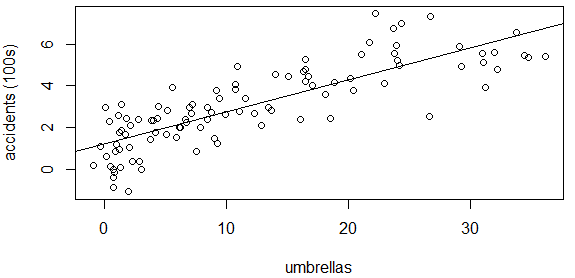
\includegraphics[width=2.5in]{umbrellas_car_accidents.png}
\end{figure}

Does 100 more umbrellas sold \textit{cause} $15.3$ more car accidents (on average)? \pause No... only an association (assessed by a linear correlation).

\end{frame}

\begin{frame}\frametitle{Correlation Does Not Imply Causation}

What can correlation mean?

\begin{itemize}
\item It is a coincidence. How can this be?
\item They are consequence from of a common cause (the \emph{lurking} or \emph{counfounding} variable). How can this be?
\item There is causation \pause
\begin{itemize}
\item x causes y (possibly with intermediates)
\item y causes x (possibly with intermediates)
\item x and y cause each other (cyclic)
\end{itemize}
(recall time-boundedness property)
\end{itemize}

\end{frame}


\begin{frame}\frametitle{Controlling for the Confounder}

The confounding variable is likely $z = $ rainfall.

\begin{figure}
\centering
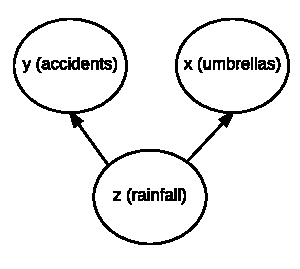
\includegraphics[width=1.5in]{confounder}
\end{figure}

The illustration shows that if you change $x$ obviously $y$ doesn't change whatsoever (causes always precede their dependent effects an assumption known as temporal boundedness) \\~\\

[Show regression in R]

\end{frame}

\begin{frame}\frametitle{A Proper Interpretation of $\betahat_j$}

$\betahat_j$ estimates $\beta_j$. Imagine $n$ is large and the confidence interval is really small. So basically, $\betahat_j = \beta_j \neq 0$. Interpretation? \\~\\ \pause

Another object naturally observed with exactly the same features except that $x_j$ is increased by $1$ unit will have a $\beta_j$ difference in its mean response $y$.\\~\\ \pause

Another one: $\betahat_j$ estimates $\beta_j$. Imagine $n$ is not so large and the confidence interval is not small but we are still convinced $\beta_j \neq 0$.  Interpretation? \\~\\

Another object naturally observed with exactly the same features except that $x_j$ is increased by $1$ unit will have a $\betahat_j \pm \se{\betahat_j}$ difference in its mean response $y$. (Not much difference except accounting for parameter estimation error).\\~\\

\end{frame}


\begin{frame}\frametitle{When can you say \qu{causes}?}

\small

When can the interpretation be as follows? \sout{Another object naturally observed with exactly the same features except for a change} \emph{If this object in front of us has its} \pause $x_j$ changed by $+1$, it will \sout{have} \emph{cause} a $\betahat_j \pm \se{\betahat_j}$ difference in its mean response $y$.

\begin{enumerate}
\item If we can just assume the model looks as follows:

\vspace{-0.3cm}

\begin{figure}
\centering
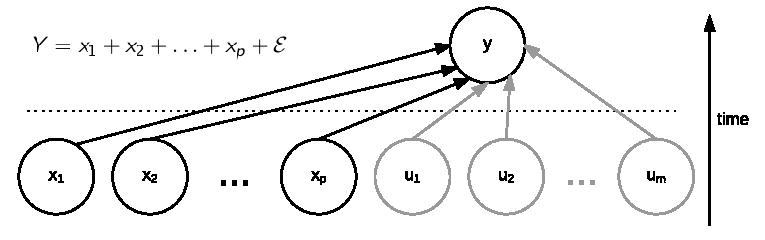
\includegraphics[width=3.5in]{get_causality}
\end{figure}

(for all $p$ features ... how can the illustration be updated for one variable?) 

\item \pause If we've run a randomized experiment manipulating $x_j$ among the objects AND assuming an additive effect of $x_j$ on $y$.
\end{enumerate}

\end{frame}

\begin{frame}\frametitle{Consider a Realistic Model}

\begin{figure}
\centering
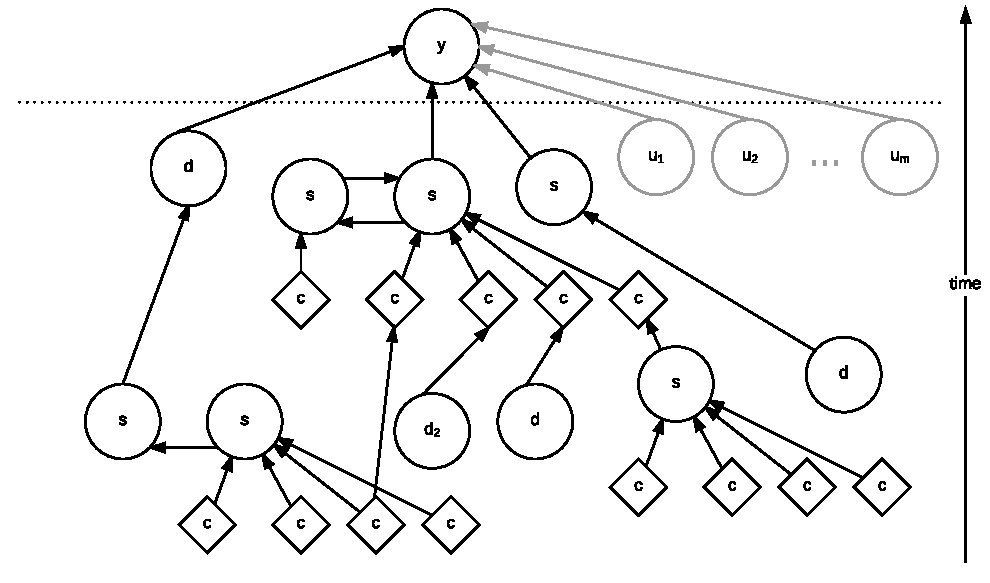
\includegraphics[width=4.5in]{realistic_model}
\end{figure}


\end{frame}

\begin{frame}\frametitle{Consider Realistic Predictors}

\begin{figure}
\centering
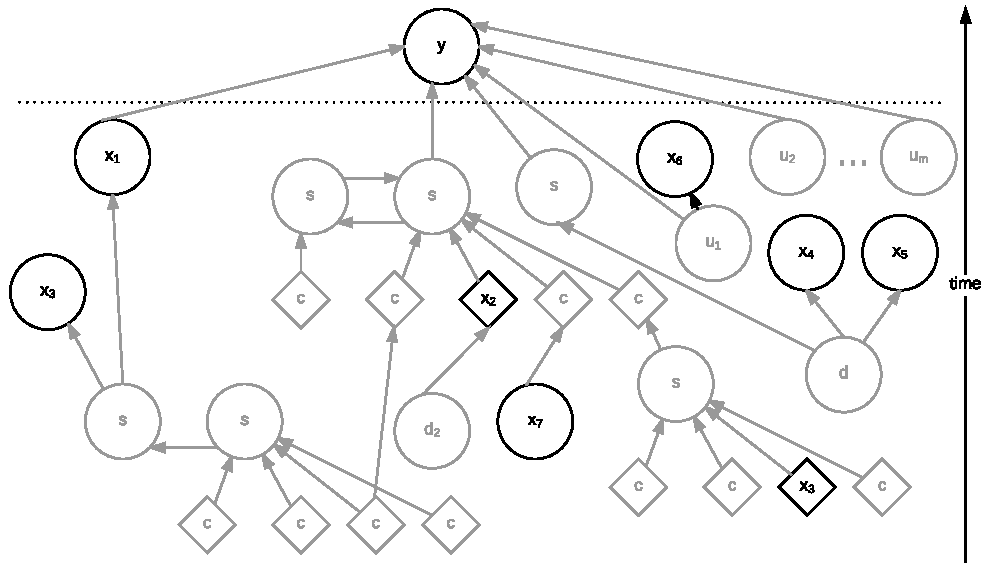
\includegraphics[width=4.5in]{realistic_predictors}
\end{figure}


\end{frame}

\begin{frame}\frametitle{Consider Realistic Predictors}

Observations from the previous illustration

\begin{itemize}
\item Maybe some of the predictors $x_1, \ldots, x_p$ are causal, but most are likely not.
\item Of the ones that are not causal due to a confounder, you may have an idea of the lurking variables but it is unlikely you can measure them. Think college GPA vs SAT with confounder true IQ / ability.
\item If some variables are causal, it is unlikely they have an additive causal effect; their effect is likely moderated by many other interacting variables possibly in non-linear ways.
\item A linear model for $y$ on $x_1, \ldots, x_p$ is likely far from the truth (not related to our discussion on causality).
\end{itemize}


\end{frame}

\begin{frame}\frametitle{More on OLS Coefficient Interpretation}

\small
The linear regression coefficient interpretation again: another object \emph{naturally observed} with exactly the same features except that $x_j$ is increased by $1$ unit will have a $\betahat_j \pm \se{\betahat_j}$ difference in its mean response $y$.\\~\\

What do we mean by naturally observed? \pause This other object is realized from the same joint distribution as all other observations. This means that whatever \textit{multicollinearity} / \textit{covariance structure} exists between the predictors, $\braces{\cov{X_j}{X_k}}$, will give rise to the predictor values in the other object.
	
\begin{figure}
\centering
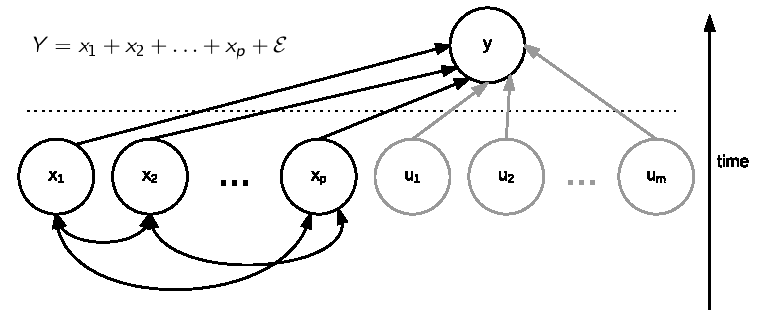
\includegraphics[width=2.8in]{predictor_covariance_structure}
\end{figure}

\end{frame}

\begin{frame}\frametitle{The Hidden \qu{Fifth} OLS Assumption}

So this language \qu{... exactly the same features except that $x_j$ is increased by ...} is kind of absurd in the context of a strong covariance structure as ... \pause it will be very rare to observe an observation with $x_j$ different without any other predictor values different. \pause Example from baseball dataset? \\~\\

There is room to argue that to have these interpretations be at all realistic, we must assume there is not a strong multicollinearity structure between $x_j$ and the other predictors.
	
\end{frame}

\begin{frame}\frametitle{But Real Correlations Still Rock}

We've been beating up on correlations and their interpretations e.g. the following:

\begin{figure}
\centering
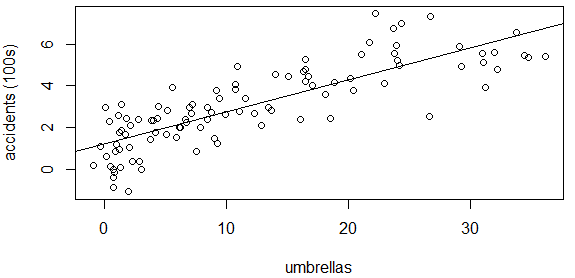
\includegraphics[width=2.5in]{umbrellas_car_accidents.png}
\end{figure}
\pause

But even though higher umbrella sales do not \qu{cause} accidents, can they still predict them? \pause Yes, $R^2$ is totally agnostic to (a) if your model is true and \pause (b) if your variables are causal or not. Predictors \textit{truly} correlated to the response contain information about the value of the response and it doesn't matter through what channel it provides that information. \pause
	
\end{frame}


\begin{frame}\frametitle{}

	
\end{frame}

\end{document}





\begin{frame}\frametitle{}

	
\end{frame}

\begin{frame}\frametitle{}

	
\end{frame}


\begin{frame}\frametitle{}

	
\end{frame}

\begin{frame}\frametitle{}

	
\end{frame}


\begin{frame}\frametitle{}

	
\end{frame}

\begin{frame}\frametitle{}

	
\end{frame}


\begin{frame}\frametitle{}

	
\end{frame}

\begin{frame}\frametitle{}

	
\end{frame}


\begin{frame}\frametitle{}

	
\end{frame}

\begin{frame}\frametitle{}

	
\end{frame}


\begin{frame}\frametitle{}

	
\end{frame}

\begin{frame}\frametitle{}

	
\end{frame}


\begin{frame}\frametitle{}

	
\end{frame}

\begin{frame}\frametitle{}

	
\end{frame}


\begin{frame}\frametitle{}

	
\end{frame}

\begin{frame}\frametitle{}

	
\end{frame}


\begin{frame}\frametitle{}

	
\end{frame}

\begin{frame}\frametitle{}

	
\end{frame}

%\begin{frame}\frametitle{$R^2$ vs. $F$ test}
%
%In this case $R^2$ will be related to $F$, the omnibus test statistic for whether the model has any signal whatsoever.
%
%\beqn
%R^2 = \frac{SSE_0 - SSE}{SSE_0} = \ldots = 1 - \inverse{1 + F \frac{p-1}{n-p}}
%\eeqn
%
%\beqn
%F &=& \frac{\frac{SSE_0 - SSE}{p - 1}}{\frac{SSE}{n-p}} = \frac{SSE_0 - SSE}{SSE} \frac{n-p}{p-1} = \ldots \\
%&=& \underbrace{\frac{R^2}{1-R^2}}_{
%%
%\substack{
%\text{ratio of variance} \\ 
%\text{explained to} \\ 
%\text{unexplained}
%}} 
%%
%\underbrace{\frac{n-p}{p-1}}_{\substack{
%\text{penalty for} \\ 
%\text{too many features}
%}}
%\eeqn